\chapter{Recurrences}\label{ch:recurrences}
Recurrences describe the running time of recursive algorithms.
Solving them---turning a recursive definition into a closed asymptotic
bound---is the central analytic step in divide-and-conquer analysis.
This chapter develops three complementary tools, highlights their limits,
and applies them to MergeSort and Karatsuba multiplication.

\section{From Algorithms to Recurrences}

A typical divide-and-conquer algorithm on input size $n$ divides into $a$ subproblems of size $n/b$, then spends $f(n)$ time dividing and combining.
\begin{figure}[htbp]
\centering
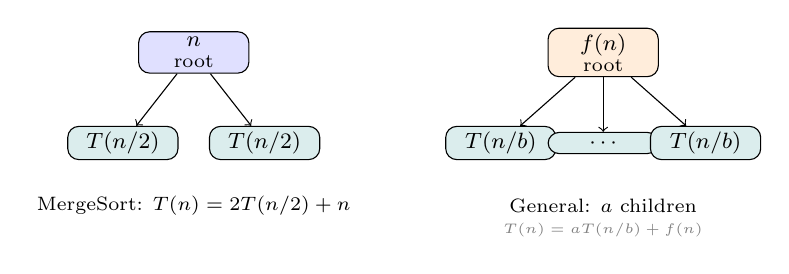
\begin{tikzpicture}[font=\footnotesize, level distance=11mm, sibling distance=16mm,
  rbox/.style={draw,rounded corners,fill=blue!12,inner sep=2pt,minimum width=14mm,align=center},
  cbox/.style={draw,rounded corners,fill=teal!14,inner sep=2pt,minimum width=14mm,align=center}]
% MergeSort instance left
\begin{scope}
\node[rbox] (mr) at (0,0) {$n$\\[-2pt]{\scriptsize root}};
\node[cbox] (m1) at (-0.9,-1.15) {$T(n/2)$};
\node[cbox] (m2) at (0.9,-1.15) {$T(n/2)$};
\draw[->,thin] (mr) -- (m1); \draw[->,thin] (mr) -- (m2);
\node[font=\scriptsize,align=center] at (0,-1.95) {MergeSort: $T(n)=2T(n/2)+n$};
\end{scope}
% General form right
\begin{scope}[xshift=5.2cm]
\node[rbox,fill=orange!14] (gr) at (0,0) {$f(n)$\\[-2pt]{\scriptsize root}};
\node[cbox] (g1) at (-1.3,-1.15) {$T(n/b)$};
\node[cbox] (g2) at (0,-1.15) {$\cdots$};
\node[cbox] (g3) at (1.3,-1.15) {$T(n/b)$};
\draw[->,thin] (gr) -- (g1); \draw[->,thin] (gr) -- (g2); \draw[->,thin] (gr) -- (g3);
\node[font=\scriptsize] at (0,-1.95) {General: $a$ children};
\node[font=\tiny,gray] at (0,-2.25) {$T(n)=aT(n/b)+f(n)$};
\end{scope}
\end{tikzpicture}
\caption{One-level expansion: peel off the root cost $f(n)$ to reveal $a$ subproblems of size $n/b$ (MergeSort instance left, general form right). Repeating this expansion yields the full recursion tree.}
\label{fig:onelevel}
\end{figure}

Its worst-case time satisfies
\begin{equation}\label{eq:general}
T(n)=a\,T(n/b)+f(n),\qquad T(1)=\Theta(1),
\end{equation}
with $a\ge 1$, $b>1$ constants and $f$ asymptotically positive. We assume $n$ is an exact power of $b$; floors and ceilings change bounds by at most a constant factor.
\textit{Running examples.} MergeSort: $T(n)=2T(n/2)+\Theta(n)$. Karatsuba (Sec.~\ref{sec:karatsuba}): $T(n)=3T(n/2)+\Theta(n)$. Binary search: $T(n)=T(n/2)+\Theta(1)$. Strassen: $T(n)=7T(n/2)+\Theta(n^{2})$.
Our goal is a $\Theta$-bound for $T(n)$---methods in order of increasing automation and decreasing generality.
\begin{remark}[Floors, ceilings, and base cases]
Replacing $T(n/b)$ by $T(\lfloor n/b\rfloor)$ or $T(\lceil n/b\rceil)$ does not change the asymptotic answer; sandwich between exact-power variants. Base cases $T(1)=\Theta(1)$ vs.\ $T(n)=O(1)$ for $n\le n_{0}$ are interchangeable up to constants.
\end{remark}

\section{The Substitution Method}

Guess a bound, then verify by induction. The method is fully general but requires insight; recursion trees (next section) are the usual source of guesses.

\smallskip\noindent\textit{Bridge---tree suggests, substitution proves.} The tree in Fig.~\ref{fig:rectree} will suggest MergeSort costs $cn$ per level $\times\log n$ levels $=cn\log n$. Here we \emph{verify} that guess rigorously; the next example shows the $cn-b$ trick when a naive guess leaves a $+1$ residue.

\begin{example}[MergeSort upper bound]
Claim $T(n)=2T(n/2)+n$ with $T(1)=1$ satisfies $T(n)=O(n\log n)$. Guess $T(n)\le cn\log n$ for $c>0$ and $n\ge 2$. Assume it holds for $n/2$:
\[T(n)\le 2c\frac{n}{2}\log\frac{n}{2}+n = cn\log n-cn+n\le cn\log n\]
provided $c\ge 1$. Choosing $c$ large enough to handle base cases completes the induction. Symmetric lower bound gives $T(n)=\Theta(n\log n)$.
\end{example}

\begin{example}[Strengthening the hypothesis]
To prove $T(n)=T(\lfloor n/2\rfloor)+T(\lceil n/2\rceil)+1$ is $O(n)$, naive $T(n)\le cn$ fails: $T(n)\le c\lfloor n/2\rfloor+c\lceil n/2\rceil+1=cn+1$. Strengthen to $T(n)\le cn-b$ for $c,b>0$:
\[T(n)\le c\lfloor n/2\rfloor-b+c\lceil n/2\rceil-b+1 = cn-2b+1\le cn-b\]
once $b\ge 1$. Subtracting a low-order term absorbs the additive constant.
\begin{center}
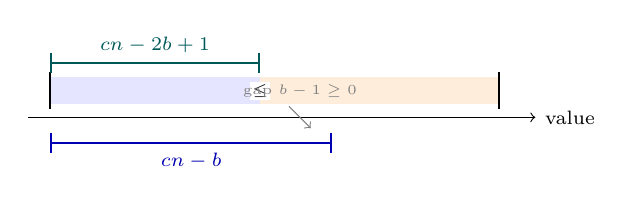
\begin{tikzpicture}[font=\scriptsize,scale=0.92]
\draw[->] (0,0) -- (7,0) node[right] {value};
\fill[blue!10] (0.3,0.18) rectangle (3.2,0.55); \fill[orange!14] (3.2,0.18) rectangle (6.5,0.55);
\draw[thick] (0.3,0.12) -- (0.3,0.62); \draw[thick] (6.5,0.12) -- (6.5,0.62);
\draw[|-|,thick,teal!70!black] (0.3,0.75) -- (3.2,0.75) node[midway,above] {$cn-2b+1$};
\draw[|-|,thick,blue!70!black] (0.3,-0.35) -- (4.2,-0.35) node[midway,below] {$cn-b$};
\node[font=\tiny,fill=white,inner sep=1pt] at (3.2,0.36) {$\le$};
\node[font=\tiny,gray] at (3.75,0.36) {gap $b-1\ge0$};
\draw[->,gray,thin] (3.6,0.15) -- (3.9,-0.15);
\end{tikzpicture}
\end{center}
\vspace{-2pt}{\scriptsize The $cn-b$ trick shifts the guess down by $b$ so the $+1$ residue is swallowed: $cn-2b+1\le cn-b\iff b\ge1$.}
\end{example}

\textit{When to use it:} only method that proves matching upper and lower bounds with full rigour, including floors. \textit{Pitfall:} guess must be tight; with floors use $n/2-1<\lfloor n/2\rfloor\le n/2$.
\paragraph{Change of variables.} For $T(n)=2T(\sqrt{n})+\log n$, set $m=\log n$, $S(m)=T(2^{m})$ to get $S(m)=2S(m/2)+m$ (MergeSort in $m$), so $S(m)=\Theta(m\log m)$ and $T(n)=\Theta(\log n\cdot\log\log n)$.

\section{The Recursion-Tree Method}

Expand the recurrence into a tree, sum level by level, then verify the guess by substitution. The tree is discovery; substitution remains the proof.
For \eqref{eq:general}, level $0$ has cost $f(n)$, level $1$ has $a$ nodes each costing $f(n/b)$, level $i$ has $a^{i}$ nodes each costing $f(n/b^{i})$. Depth $L=\log_{b}n$,
\begin{equation}\label{eq:treesum}
T(n)=\sum_{i=0}^{L-1} a^{i}f(n/b^{i})+\Theta(n^{\log_{b}a}),
\end{equation}
where last term is leaf cost ($a^{L}=n^{\log_{b}a}$ leaves each $\Theta(1)$). Bounding this sum is the entire problem. Fig.~\ref{fig:rectree} illustrates the expansion.
\begin{figure}[htbp]
\centering
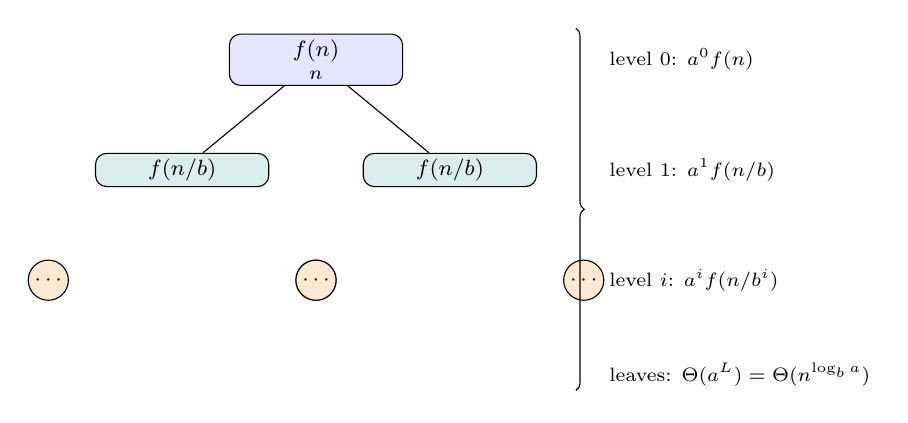
\begin{tikzpicture}[
  level distance=14mm, sibling distance=34mm,
  every node/.style={font=\footnotesize},
  rnode/.style={draw,rounded corners,fill=blue!10,inner sep=2pt,minimum width=22mm,align=center},
  rnodeB/.style={draw,rounded corners,fill=teal!14,inner sep=2pt,minimum width=22mm,align=center},
  leaf/.style={draw,circle,fill=orange!18,inner sep=1.5pt}
]
\node[rnode] (root) {$f(n)$\\[-1pt]{\scriptsize $n$}}
  child {node[rnodeB] {$f(n/b)$}
    child {node[leaf] {$\cdots$} edge from parent[draw=none]}
    child {node[leaf] {$\cdots$} edge from parent[draw=none]}
  }
  child {node[rnodeB] {$f(n/b)$}
    child {node[leaf] {$\cdots$} edge from parent[draw=none]}
    child {node[leaf] {$\cdots$} edge from parent[draw=none]}
  };
\node[anchor=west,font=\scriptsize] at (3.6,0) {level $0$: $a^{0}f(n)$};
\node[anchor=west,font=\scriptsize] at (3.6,-1.4) {level $1$: $a^{1}f(n/b)$};
\node[anchor=west,font=\scriptsize] at (3.6,-2.8) {level $i$: $a^{i}f(n/b^{i})$};
\node[anchor=west,font=\scriptsize] at (3.6,-4.0) {leaves: $\Theta(a^{L})=\Theta(n^{\log_{b}a})$};
\draw[decorate,decoration={brace,amplitude=3pt},thin] (3.3,0.4) -- (3.3,-4.2);
\end{tikzpicture}
\caption{Recursion tree for $T(n)=aT(n/b)+f(n)$. Total cost is sum over levels plus leaves; $L=\log_{b}n$.}
\label{fig:rectree}
\end{figure}

\begin{example}[MergeSort via tree]
$T(n)=2T(n/2)+cn$. Level $i$ has $2^{i}$ nodes of cost $cn/2^{i}=cn$, so each level costs $cn$. With $\log_{2}n$ levels, $T(n)=cn\log_{2}n+\Theta(n)=\Theta(n\log n)$.
\end{example}

\begin{example}[Karatsuba preview]
$T(n)=3T(n/2)+cn$. Level $i$ costs $3^{i}\cdot c(n/2^{i})=cn(3/2)^{i}$---geometric, ratio $3/2>1$, dominated by last term:
\[\sum_{i=0}^{L-1}cn(3/2)^{i}=cn\frac{(3/2)^{L}-1}{3/2-1}=\Theta(n\cdot n^{\log_{2}3-1})=\Theta(n^{\log_{2}3}).\]
The Master theorem automates this.
\end{example}

\begin{remark}
Trees handle recurrences outside the Master form, e.g.\ $T(n)=T(n/3)+T(2n/3)+\Theta(n)$, where longest path is $\log_{3/2}n$ and careful bounding still yields $\Theta(n\log n)$---settled directly by Akra--Bazzi. In general, if $a^{i}f(n/b^{i})$ grows (resp.\ shrinks) by a constant factor each level, the sum is dominated by the last (resp.\ first) term.
\end{remark}
\paragraph{Recurrence with non-constant work.} $T(n)=2T(n/2)+n\log n$: level $i$ has $2^{i}$ nodes each $(n/2^{i})\log(n/2^{i})$, so level cost $n(\log n-i)$. Summing gives $n\sum_{i=0}^{L-1}(\log n-i)=\Theta(n\log^{2}n)$, matching Master Case~2 with $k=1$.

\section{The Master Theorem}\label{sec:master}

The Master theorem classifies \eqref{eq:general} when $f$ is polynomially comparable to $n^{\log_{b}a}$. It replaces tree summation with a case check.

\begin{figure}[htbp]
\centering
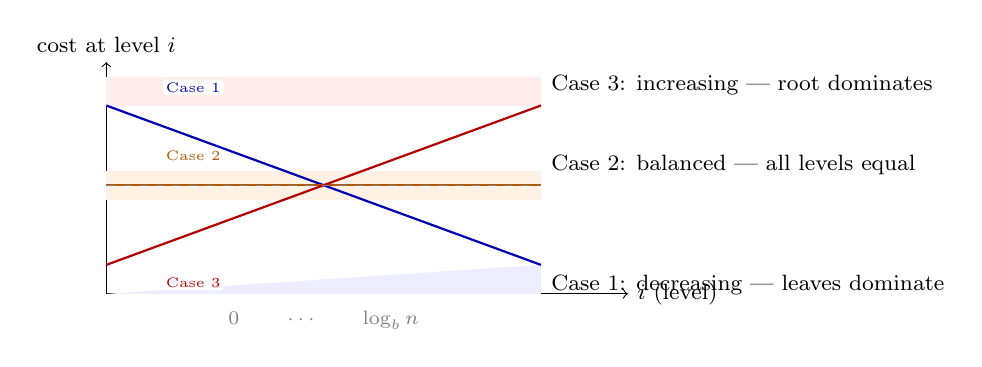
\begin{tikzpicture}[scale=0.92,font=\footnotesize]
\draw[->] (0,0) -- (7.2,0) node[right] {$i$ (level)};
\draw[->] (0,0) -- (0,3.2) node[above] {cost at level $i$};
\fill[blue!7] (0,0) -- (6,0.4) -- (6,0) -- (0,0) -- cycle;
\fill[red!7] (0,2.6) -- (6,2.6) -- (6,3.0) -- (0,3.0) -- cycle;
\fill[orange!10] (0,1.3) rectangle (6,1.7);
\draw[thick,blue!70!black] (0,2.6) -- (6,0.4) node[anchor=north west,black] {Case 1: decreasing --- leaves dominate};
\draw[thick,orange!70!black] (0,1.5) -- (6,1.5) node[anchor=south west,black] {Case 2: balanced --- all levels equal};
\draw[thick,red!70!black] (0,0.4) -- (6,2.6) node[anchor=south west,black] {Case 3: increasing --- root dominates};
\draw[dashed,gray] (0,1.5) -- (6,1.5);
\node[font=\tiny, fill=white, rounded corners=1pt, inner sep=1pt] at (1.2,2.85) {\color{blue!70!black}Case 1};
\node[font=\tiny, fill=white, rounded corners=1pt, inner sep=1pt] at (1.2,1.9) {\color{orange!70!black}Case 2};
\node[font=\tiny, fill=white, rounded corners=1pt, inner sep=1pt] at (1.2,0.15) {\color{red!70!black}Case 3};
\node[anchor=north,font=\scriptsize,gray] at (3,-0.1) {$0\qquad\cdots\qquad \log_{b}n$};
\end{tikzpicture}
\caption{Master geometry: per-level cost $a^{i}f(n/b^{i})$ across levels. The dominant contribution determines the case---read the picture before the theorem.}
\label{fig:mastergeom}
\end{figure}

\textit{Walk-through (Fig.~\ref{fig:mastergeom}).} Plot $a^{i}f(n/b^{i})$ versus $i$. \textbf{Shrinking} (blue, Case~1): level cost falls geometrically, last level $\approx n^{c_{\star}}$ dominates, so $T(n)=\Theta(n^{c_{\star}})$---e.g.\ Karatsuba $3T(n/2)+n$. \textbf{Flat} (orange, Case~2): every level contributes $\Theta(n^{c_{\star}})$, $\log_{b}n$ levels give $\Theta(n^{c_{\star}}\log n)$---e.g.\ MergeSort $2T(n/2)+n$. \textbf{Increasing} (red, Case~3): cost grows geometrically, root $f(n)$ dominates, so $T(n)=\Theta(f(n))$ provided regularity $af(n/b)\le cf(n)$ forces geometric decay upward.

\begin{theorem}[Master theorem]\label{thm:master}
Let $a\ge 1$, $b>1$, $f$ asymptotically positive, and $T(n)=aT(n/b)+f(n)$. Let $c_{\star}=\log_{b}a$.
\begin{enumerate}[label=Case~\arabic*:,leftmargin=*]
\item If $f(n)=O(n^{c_{\star}-\varepsilon})$ for some $\varepsilon>0$, then $T(n)=\Theta(n^{c_{\star}})$.
\item If $f(n)=\Theta(n^{c_{\star}}\log^{k}n)$ for some $k\ge 0$, then $T(n)=\Theta(n^{c_{\star}}\log^{k+1}n)$. In particular $f(n)=\Theta(n^{c_{\star}})$ gives $\Theta(n^{c_{\star}}\log n)$.
\item If $f(n)=\Omega(n^{c_{\star}+\varepsilon})$ for some $\varepsilon>0$ and the \emph{regularity} condition $af(n/b)\le cf(n)$ holds for some $c<1$ and large $n$, then $T(n)=\Theta(f(n))$.
\end{enumerate}
\end{theorem}
\paragraph{Proof sketch.} Write $g(n)=f(n)/n^{c_{\star}}$ so $a^{i}f(n/b^{i})=n^{c_{\star}}g(n/b^{i})$. Then \eqref{eq:treesum} $=n^{c_{\star}}\sum_{i}g(n/b^{i})+\Theta(n^{c_{\star}})$.
Case~1: $g(n)=O(n^{-\varepsilon})$, sum is convergent geometric $\Rightarrow\Theta(n^{c_{\star}})$.
Case~2: $g(n)=\Theta(\log^{k}n)$, sum over $L=\Theta(\log n)$ terms $\Rightarrow\Theta(\log^{k+1}n)$.
Case~3: regularity gives $a^{i}f(n/b^{i})\le c^{i}f(n)$, geometric decay toward leaves, sum $=\Theta(f(n))$.
\paragraph{Why regularity is needed.} Without it Case~3 is false: contrived $f$ with $f(n)=\Omega(n^{c_{\star}+\varepsilon})$ can dip sharply at infinitely many $n/b^{i}$, breaking geometric decay. For polynomials it is automatic---check $af(n/b)/f(n)=a/b^{k}<1$ when $f(n)=n^{k}$, $k>c_{\star}$.
\paragraph{Gaps.} The theorem does \emph{not} cover every $f$. Need $\varepsilon>0$ polynomial gap: $f(n)=n^{c_{\star}}\log\log n$ and $f(n)=n^{c_{\star}}/\log n$ fall strictly between Cases~1 and~2.

\noindent\fbox{\begin{minipage}{0.96\linewidth}\footnotesize\textbf{Gap box ($n=1024$).} Take $c_{\star}=2$ so $n^{c_{\star}}=1\,048\,576$. Then $n^{c_{\star}}/\log_{2}n = 1\,048\,576/10 = 104\,858$ while $n^{c_{\star}}\log\log n\approx 1\,048\,576\times 3.32\approx 3.48$M. Neither is $O(n^{2-\varepsilon})$ nor $\Omega(n^{2+\varepsilon})$ nor $\Theta(n^{2})$ for any fixed $\varepsilon>0$; the ratio $f(n)/n^{c_{\star}}=1/\log n$ (or $\log\log n$) tends to $0$ (or $\infty$) slower than any $n^{\pm\varepsilon}=1024^{\pm\varepsilon}$. Hence no Master case applies---use tree/Akra--Bazzi. The true cost is \emph{between} $n^{c_{\star}}$ and $n^{c_{\star}}\log n$.\end{minipage}}
\paragraph{How to apply it.} (1) Compute $c_{\star}=\log_{b}a$. (2) Compare $f(n)$ to $n^{c_{\star}}$: polynomially smaller / Theta-equivalent (up to $\log^{k}n$) / polynomially larger with regularity? (3) If none holds, Master is silent---use tree or Akra--Bazzi.

\subsection{Worked Applications}
\paragraph{MergeSort.} $a=2$, $b=2$, $c_{\star}=1$, $f(n)=\Theta(n)=\Theta(n^{c_{\star}})$: Case~2 $\Rightarrow\Theta(n\log n)$.
\paragraph{Karatsuba.}\label{sec:karatsuba} $n$-digit $X=a\cdot10^{m}+b$, $Y=c\cdot10^{m}+d$, $m=n/2$. Three products suffice: $T(n)=3T(n/2)+\Theta(n)$. Here $c_{\star}=\log_{2}3\approx1.585$, $f(n)=O(n^{c_{\star}-0.58})$: Case~1 $\Rightarrow\Theta(n^{\log_{2}3})$, beating naive $\Theta(n^{2})$.
\paragraph{Strassen.} $T(n)=7T(n/2)+\Theta(n^{2})$: $c_{\star}=\log_{2}7\approx2.807>2$, Case~1 $\Rightarrow\Theta(n^{\log_{2}7})$.
\paragraph{Binary search.} $T(n)=T(n/2)+\Theta(1)$: $c_{\star}=0$, $f(n)=\Theta(1)$: Case~2 $\Rightarrow\Theta(\log n)$.
\paragraph{Quick check.} $T(n)=9T(n/3)+\Theta(n^{2})$: $c_{\star}=2$, $f=\Theta(n^{c_{\star}})$ so Case~2 $\Rightarrow\Theta(n^{2}\log n)$; $f=n^{3}\Rightarrow$ Case~3; $f=n\Rightarrow$ Case~1.

\begin{table}[htbp]
\centering\small
\begin{tabular}{@{}llll@{}}
\toprule
Relation of $f(n)$ to $n^{c_{\star}}$ & Case & $T(n)$ & Intuition \\
\midrule
$f(n)=O(n^{c_{\star}-\varepsilon})$ & 1 & $\Theta(n^{c_{\star}})$ & Leaves dominate \\
$f(n)=\Theta(n^{c_{\star}}\log^{k}n)$ & 2 & $\Theta(n^{c_{\star}}\log^{k+1}n)$ & Balanced levels \\
$f(n)=\Omega(n^{c_{\star}+\varepsilon})$, regular & 3 & $\Theta(f(n))$ & Root dominates \\
Gaps: $n^{c_{\star}}/\!\log n$, $n^{c_{\star}}\log\log n$ & --- & --- & Use tree / Akra--Bazzi \\
\bottomrule
\end{tabular}
\caption{Master theorem at a glance ($c_{\star}=\log_{b}a$). Memory aid---still check $\varepsilon$ and regularity.}
\label{tab:master}
\end{table}

\section{Beyond Equal Subproblems: Akra--Bazzi}

\begin{figure}[htbp]
\centering
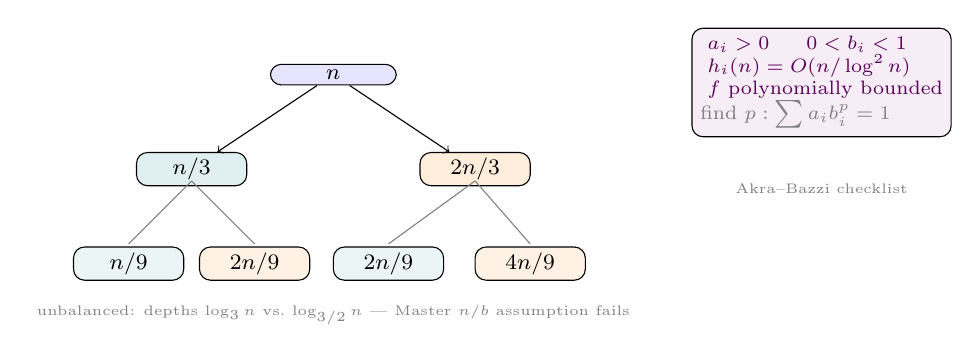
\begin{tikzpicture}[font=\footnotesize, level distance=10mm, sibling distance=18mm,
  rbox/.style={draw,rounded corners,fill=blue!10,inner sep=2pt,minimum width=16mm,align=center},
  cbox/.style={draw,rounded corners,fill=teal!12,inner sep=2pt,minimum width=14mm,align=center},
  cbox2/.style={draw,rounded corners,fill=orange!14,inner sep=2pt,minimum width=14mm,align=center}]
% Lopsided tree
\node[rbox] (r) at (0,0) {$n$};
\node[cbox] (a) at (-1.8,-1.2) {$n/3$};
\node[cbox2] (b) at (1.8,-1.2) {$2n/3$};
\draw[->,thin] (r)--(a); \draw[->,thin] (r)--(b);
\node[cbox,fill=teal!8] at (-2.6,-2.4) {$n/9$}; \node[cbox2,fill=orange!10] at (-1.0,-2.4) {$2n/9$};
\node[cbox,fill=teal!8] at (0.7,-2.4) {$2n/9$}; \node[cbox2,fill=orange!10] at (2.5,-2.4) {$4n/9$};
\draw[thin,gray] (-2.6,-2.15)--(-1.8,-1.35); \draw[thin,gray] (-1.0,-2.15)--(-1.8,-1.35);
\draw[thin,gray] (0.7,-2.15)--(1.8,-1.35); \draw[thin,gray] (2.5,-2.15)--(1.8,-1.35);
\node[font=\tiny,gray] at (0,-3.05) {unbalanced: depths $\log_{3}n$ vs.\ $\log_{3/2}n$ --- Master $n/b$ assumption fails};
% Checklist on right
\begin{scope}[xshift=6.2cm,yshift=-0.1cm]
\node[draw,rounded corners,fill=violet!7,inner sep=3pt,align=left,font=\scriptsize] (chk) {
\color{violet!70!black}$\checkmark$ $a_i>0$ \quad $\checkmark$ $0<b_i<1$\\
\color{violet!70!black}$\checkmark$ $h_i(n)=O(n/\log^{2}n)$\\
\color{violet!70!black}$\checkmark$ $f$ polynomially bounded\\
\color{gray} find $p:\sum a_i b_i^{p}=1$
};
\node[font=\tiny,gray,align=center] at (0,-1.35) {Akra--Bazzi checklist};
\end{scope}
\end{tikzpicture}
\caption{Lopsided recursion for $T(n)=T(n/3)+T(2n/3)+\Theta(n)$ and Akra--Bazzi applicability checklist.}
\label{fig:akra}
\end{figure}

When subproblem sizes differ or $f$ is not polynomially separated, Master does not apply. Akra--Bazzi handles
\[T(n)=\sum_{i=1}^{k}a_{i}T(b_{i}n+h_{i}(n))+f(n),\quad 0<b_{i}<1,\ a_{i}>0,\]
with $h_{i}(n)=O(n/\log^{2}n)$. Let $p$ solve $\sum_{i}a_{i}b_{i}^{p}=1$. Then
\[T(n)=\Theta\!\left(n^{p}\Bigl(1+\int_{1}^{n}\frac{f(u)}{u^{p+1}}\,du\Bigr)\right).\]
For Master form $aT(n/b)+f(n)$ this recovers all three cases. For $T(n)=T(n/3)+T(2n/3)+\Theta(n)$ we get $p=1$ and $\int_{1}^{n}u^{-1}du=\log n$, so $T(n)=\Theta(n\log n)$. Check: $T(n)=2T(n/4)+\Theta(\sqrt{n})$ has $2(1/4)^{p}=1\Rightarrow p=1/2$, $\int u^{1/2}/u^{3/2}du=\log n$, so $\Theta(\sqrt{n}\log n)$, matching Master Case~2.

\begin{remark}[Using Akra--Bazzi in SC2001]
You may quote it without reproving, but verify hypotheses: $a_{i}>0$, $0<b_{i}<1$, $h_{i}(n)=O(n/\log^{2}n)$, $f$ polynomially bounded. For $T(n)=T(n/2)+T(n/4)+\Theta(n)$, $(1/2)^{p}+(1/4)^{p}=1\Rightarrow p\approx0.694$; integral is $\Theta(n)$-dominated $\Rightarrow T(n)=\Theta(n)$.
\end{remark}

\section{Chapter Notes and Exercises}
Substitution builds proof discipline; trees build intuition; Master automates the common case. Table~\ref{tab:master} summarises. When subproblems are unequal, floors are messy, or $f$ oscillates, fall back to trees or Akra--Bazzi. Habit: conjecture with tree, confirm dominant case with Master when applicable, verify by substitution.

\begin{exercise}[Substitution practice]
Solve $T(n)=4T(n/2)+n$ with $T(1)=1$. Guess $T(n)=O(n^{2})$ and prove by substitution. Then prove $\Omega(n^{2})$ to conclude $\Theta(n^{2})$. Which Master case?
\end{exercise}
\begin{exercise}[Recursion tree]
Use a tree to conjecture bounds for (a) $T(n)=2T(n/2)+n^{2}$ and (b) $T(n)=T(n/2)+T(n/4)+\Theta(n)$. Verify one by substitution. For which does Master apply?
\end{exercise}
\begin{exercise}[Master theorem gaps]
For each state which Master case applies (or why none) and give bound: (a) $T(n)=2T(n/2)+n\log n$, (b) $T(n)=2T(n/2)+n/\log n$, (c) $T(n)=4T(n/2)+n^{2}\log n$, (d) $T(n)=2T(n/2)+\Theta(n^{1.5})$.
\end{exercise}
\begin{exercise}[Karatsuba vs.\ naive]
Karatsuba $T_{K}(n)=3T_{K}(n/2)+\Theta(n)$ vs.\ naive $T_{N}(n)=4T_{N}(n/2)+\Theta(n)$. Compute both bounds and find smallest $n=2^{k}$ where $n^{\log_{2}3}<n^{2}/10$.
\end{exercise}
